\documentclass[preprint,12pt]{elsarticle}
\usepackage{etex}


\makeatletter
\providecommand{\doi}[1]{%
	\begingroup
	\let\bibinfo\@secondoftwo
	\urlstyle{rm}%
	\href{http://dx.doi.org/#1}{%
		doi:\discretionary{}{}{}%
		\nolinkurl{#1}%
	}%
	\endgroup
}
\makeatother
%\usepackage{natbib}
% encoding and languages
\usepackage{hyperref}
\usepackage[utf8]{inputenc}
\usepackage[T1]{fontenc}
\usepackage[ngerman,english]{babel}
\usepackage{wrapfig}
\usepackage{times}
\usepackage{paralist}
\usepackage{graphicx, color}
%\usepackage{subfigure}
\usepackage{subfig}
%\usepackage{subfloat}
\usepackage{booktabs}
\usepackage{caption}
%\usepackage{subcaption}
\usepackage{paralist}
\usepackage{amssymb, amsfonts}
\usepackage{amsmath}
%\usepackage{amsthm}
\usepackage{amsopn}
\newtheorem{myProb}{Problem}
\newtheorem{mythm}{Theorem}

\newtheorem{myproof}{Proof}
\newtheorem{mysketch}{Proof Sketch}
%\usepackage[ruled]{algorithm2e}
%\usepackage[colorinlistoftodos]{todonotes}
%\usepackage{qtree}
\usepackage{tikz, tikz-qtree}
\usepackage[ruled]{algorithm2e}
%\usepackage{Algorithmic}
\usepackage{times}
\usepackage{microtype}
\usepackage{url}
\usepackage{balance}
\let\proof\relax 
\let\endproof\relax
\usepackage{multirow}
\usepackage{relsize}
\usepackage{caption}
\usepackage{color, colortbl}
\usepackage{array, booktabs, ragged2e}
\usepackage{makecell}
\usepackage{tikz}
\usepackage{textpos}

\usepackage{pdflscape}
\newcommand{\RNum}[1]{\uppercase\expandafter{\romannumeral #1\relax}}

\graphicspath{{./Figures/}}

\newcommand{\mypar}[1]{\smallskip\noindent\textbf{#1.}}

\newtheorem{prob}{Problem}


\newtheorem{mydef}{Definition}
%\newtheorem{remark}{Remark}

\newcommand{\todo}[1]{{\textcolor{red}{\bf {#1}}}}

%\newcommand{\mytitle}{Exploiting Software and Hardware Advances  in Optimization Methods for Improved Wind Farm Design}
\newcommand{\mytitle}{Exploiting Hardware and Software Advances 
 for Quadratic Models of Wind Farm Layout Optimization}
%\newcommand{\mytitlerunning}{\mytitle}
%\newcommand{\myauthor}{Arik Senderovich, Eldan Cohen, and J. Christopher Beck}
%\newcommand{\myauthorhyperref}{Arik Senderovich, Eldan Cohen, and J. Christopher Beck}


%\hypersetup{
%    bookmarks=true,        % show bookmarks bar?
%    unicode=true,          % non-latin characters in bookmarks?
%    pdffitwindow=false,    % window fit to page when opened
%    pdfstartview={FitH},   % fits width of the page to the window
%    pdftoolbar=true,       % show acrobat toolbar?
%    pdfmenubar=true,       % show acrobat menu?
%    colorlinks=true,      % false: boxed links; true: color links
%    linkcolor={blue!80!black},       % color of internal links
%    urlcolor={blue!30!black},        % color of external links
%    citecolor={green!60!black},       % color of links to bibliography
%    filecolor=black,       % color of file links
%    pdftitle={\mytitle},           % title
%    pdfauthor={\myauthorhyperref}, % author
%    pdfcreator={\myauthorhyperref} % creator of pdf
%}

\begin{document}
	

\title{\mytitle}

%\subtitle{Extended Abstract}
%\author{}
%\institute{}
%\author{\myauthor}
%\institute{Department of Mechanical and Industrial Engineering, University of Toronto\\
%\email{sariks@mie.utoronto.ca, ecohen@mie.utoronto.ca, jcb@mie.utoronto.ca}}


\author[add1]{Arik Senderovich}

%\ead[url]{https://ischool.utoronto.ca/profile/arik-senderovich/}
\ead{arik.senderovich@utoronto.ca}

\author[add2]{Eldan Cohen}
\ead{ecohen@mie.utoronto.ca}
%\ead[url]{homepageldan}




%\address[1]{}



%\address[2]{40 St. George St., Toronto, Canada}
\author[add2]{Jiachen Zhang}
\ead{jasonzjc@mie.utoronto.ca}

\author[add2]{J. Christopher Beck\corref{cor1}}
\ead{jcb@mie.utoronto.ca}


%\ead[url]{homepageldan}
%\address[3]{}
\address[add1]{Faculty of Information, University of Toronto, 140 St. George St., Toronto, Canada}
\cortext[cor1]{Corresponding author}
\address[add2]{Department of Mechanical and Industrial Engineering, University of Toronto, 40 St. George St., Toronto, Canada}

\begin{abstract} 
%Wind farms play an increasingly important
%role as a source of renewable energy and 
  A key aspect of the design of a wind farm is the wind farm layout optimization (WFLO) problem: given a wind farm site, decide the location of individual wind turbines to maximize energy production subject to proximity restrictions and wake-based interference among turbines. Given the pairwise wake interactions, it is natural
%While a number of heuristic and exact techniques have been proposed to solve WFLO, it is common
to model the energy objective as a quadratic function as, indeed, has been done in some existing optimization models. Recent advances in both optimization hardware and software have targeted quadratic constraints: commercial mixed integer linear solvers have been extended to address some quadratic problems and nascent specialized hardware, including quantum computing systems, have focused on solving quadratic unconstrained binary optimization (QUBO) problems. 
%It is a key problem 
%when designing a new wind farm, as it has a direct influence
%on the amount of the total produced energy. 
%In recent years there have been advances in both software technologies (e.g., the extension of commercial mixed integer linear programming solvers to handle quadratic problems) and nascent hardware development (e.g., quantum computing chips and specialized classical chips) that have relevance for the WFLO problem. In both cases, the advances have 
%Recent years saw 
%advances in software and hardware optimization technologies, such as Gurobi's quadratic solver 
%and Fujitsu's digital annealer (DA), respectively. 
%These technologies create an opportunity to improve 
%over current wind farm optimization solutions
%both in terms of solution quality and solve time. 
%In order to exploit these technologies, 
%we must represent the WFLO problem as 
%a quadratic optimization model. Specifically, in order 
%to apply a software-based optimization
%solution (Gurobi), 
In this paper, we 
introduce two novel quadratic programming models for WFLO: a quadratic constrained optimization problem (QCOP) with binary decision variables and a QUBO.
%Subsequently, we provide the unconstrained counterpart of the QCOP, 
%namely the quadratic unconstrained binary optimization (QUBO), which  
%is the underlying representation for quantum-inspired 
%optimization hardware such as the DA. 
A thorough empirical 
evaluation using a commercial solver and specialized QUBO hardware
%demonstrates the strengths of the two models. 
%Our results
show that both approaches yield fast, high-quality solutions 
that
improve the state of the art. In particular, the QUBO model delivers high quality solutions very quickly while the QCOP model can be used to find better solutions and provide quality guarantees over a longer run-time.
\end{abstract}
\begin{keyword}
	Wind Farm Layout Optimization (WFLO) \sep Quadratic Programming (QP) \sep Quadratic Unconstrained Binary Optimization (QUBO) \sep Digital Annealer
\end{keyword}

\maketitle 

\section{Introduction}
% Todo
The goal in the wind farm layout optimization (WFLO)
problem~\cite{MOSETTI1994105} is to locate wind turbines within a
predefined area to maximize the total power harvested from the wind
stream.  While physical considerations based on the diameter of the
blades prevent turbines being placed too close to each other, turbine
location decisions influence the total power production due to
interference effects (i.e., wakes) generated by upstream turbines.
These inter-turbine effects are best captured by Jensen's wake model~\cite{jensen1983note} when superimposed
using a sum-of-squares expression~\cite{Zhang2014}. However,
this wake modeling yields intractable optimization problems
that must be approximated using either quadratic or linear functions~\cite{turner2014new}.
An alternative formulation of WFLO relies on a less accurate wake model, which uses linear superpositioning
to capture multiple wakes~\cite{donovan2005wind}.
The latter can be captured using quadratic
constraints and objective functions. However, exact optimization
approaches that have been proposed for the alternative WFLO formulation~\cite{Zhang2014,kuo2016wind,donovan2005wind,fagerfjall2010optimizing,archer2011wind,sorkhabi2018constrained}
represent the quadratic relations using approximate linear models,
%that approximate wake dependencies,
as, until recent years, solving quadratic programming problems
was computationally challenging compared to linear models.

In this work, we introduce two novel quadratic WFLO models. The first
model represents WFLO as a quadratic constrained optimization
problem (QCOP).  The QCOP can be solved quickly using state-of-the-art mathematical solvers
that have been recently extended for such problems, e.g., Gurobi~\cite{gurobi}.  Our
second model is a quadratic unconstrained binary optimization
(QUBO) representation of the WFLO problem.  Such a formulation enables the use of
nascent specialized optimization hardware tailored to solve QUBOs: we use Fujitsu's Digital Annealer (DA) \cite{aramon2019physics} here.
%, a hardware-based
%QUBO solver, to demonstrate the strength of our approach.

The main
contributions of this paper are:
\begin{enumerate} 
\item We propose a novel quadratic modeling framework for WFLO that encompasses both constrained and unconstrained quadratic optimization models.
 %that captures wake 
%effects directly through their linear superposition. 
%without the need for approximations and ad-hoc solutions,
\item We prove that WFLO is $\mathcal{NP}$-hard.
\item Through numerical experiments on two instantiations of our quadratic framework using Fujitsu's Digital Annealer and a commercial software-based quadratic solver (Gurobi), we demonstrate state-of-the-art performance in, respectively, quickly finding high-quality solutions and finding and proving optimal solutions over a longer run-time.
\end{enumerate}

Our experiments are focused on the performance of the two approaches
compared to 
existing optimization methods. To this end,
we experiment with 12 standard WFLO benchmark problems (c.f.~\cite{turner2014new})
and show that solving quadratic WFLO models
using Gurobi and the DA
achieves state-of-the-art performance.
%, often outperforming existing solutions when provided sufficient run-time.
Furthermore, we observe that the DA 
often provides solutions of similar quality two orders of magnitude faster
than software-based approaches.

The remainder of this paper is structured as follows. Section~\ref{sec:related} presents our wind farm model and a literature review of exact and approximate
optimization solutions to the layout problem. The main contribution, namely the two quadratic models, is introduced in Section~\ref{sec:QUBO4WFLO} and Section~\ref{sec:eval} demonstrates the value of our approach via a thorough empirical evaluation.
%of the proposed methods. 
Lastly, Section~\ref{sec:conclusion} provides concluding remarks and directions for future work.   


\section{Background}
\label{sec:related}

We start this section by presenting the physical model of a wind farm
used throughout the paper.  Our wind farm model is based on the common
notation and description presented in~\cite{Zhang2014}.  Subsequently,
we provide a literature review of existing mathematical optimization
methods for solving WFLO, focusing on their similarities and
differences with our approach.
 
\subsection{The Wind Farm Model}

%\paragraph{Wind Farm as a Grid}
We consider a square-shaped wind farm that we model as an $n\times n$
grid with $n$ being the number of cells on each axis.  The cells have
an area of $c^2$ (in squared meters), i.e., if $c=100$ meters and
$n=20$, the farm area will be $2km\times 2km$.  In this work, we
assume that the terrain is flat and that we have no constraints
related to the terrain.  Furthermore, we do not account for the
influence of noise on the wind farm's surroundings. The wind farm
literature treats the more complex farm models that capture non-flat
terrain~\cite{song2015lazy,kuo2016wind}, multi-typed
turbines~\cite{feng2017design}, noise
effects~\cite{Zhang2014,sorkhabi2016impact,yin2014multi}, and complex
objectives (including turbine installation and maintenance
costs)~\cite{lackner2007analytical,sorkhabi2018constrained}.  In this work, we focus on the
novel quadratic approach for WFLO, and hence consider the most
abstract wind farm model. Our model can be extended, in the
future, to include additional wind farm settings. 
 
We assume that the number of identical turbines to be placed is known 
in advance and denote the number of turbines by $m$. To place these $m$ turbines, 
we must consider two types of interference effects, namely \emph{proximity constraints} and \emph{wakes}.
In what follows, we explain the two effects using a toy example of placing a single turbine on an 
$8\times8$ grid (see Figure~\ref{fig:field_model}).

\begin{figure}[t]
	\centering
	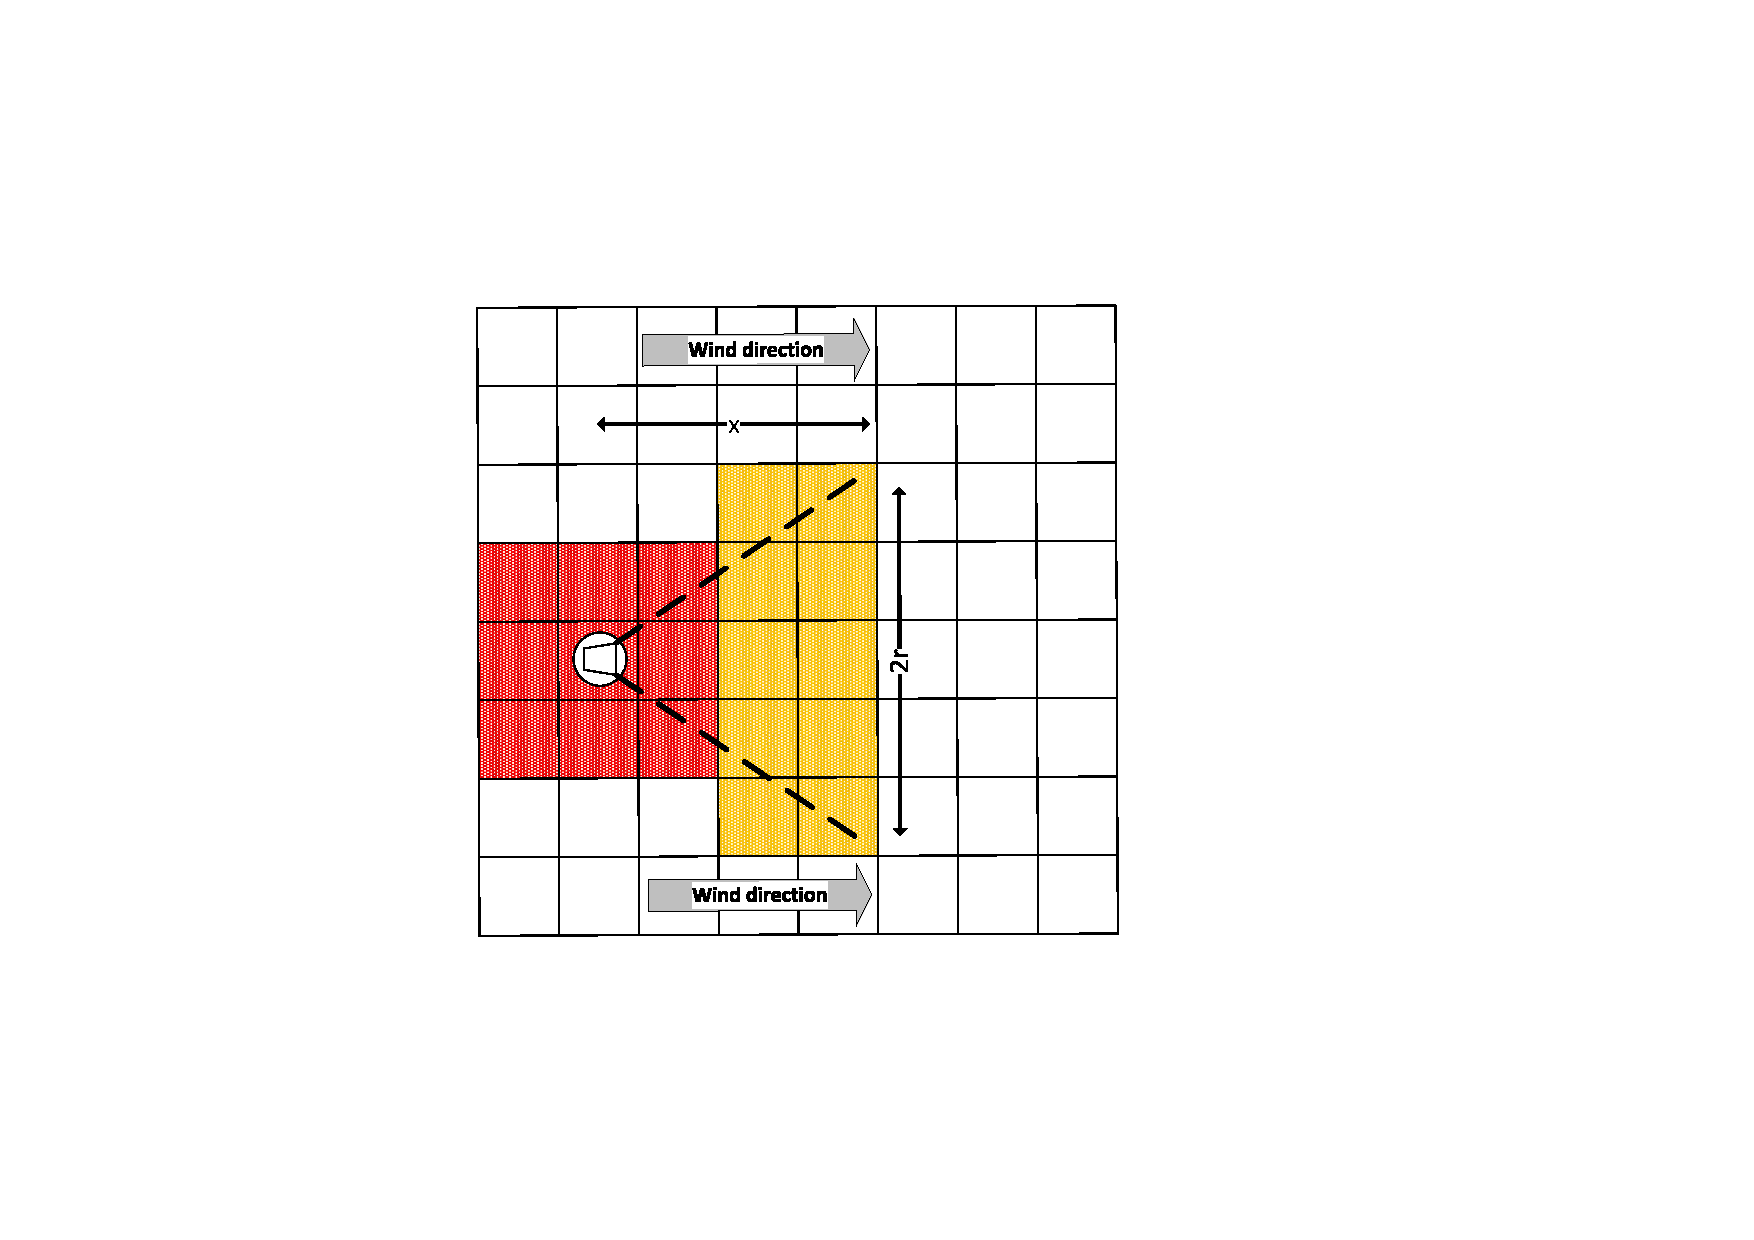
\includegraphics[scale = 0.9]{field_model.pdf}

	\caption{Wind farm model: proximity constraints, wakes, wind direction.}\label{fig:field_model}
\end{figure}



\paragraph{Proximity Constraints}
Turbines must be placed at least \emph{five rotor diameters}
apart. Depending on the cell size, we shall formulate the
corresponding constraint as part of the optimization model. For
example, assume that a turbine is placed in the center of a
cell. Then, given a cell size of $c = 100$ meters and a rotor diameter
of $40$ meters, we must ensure that two turbines are not placed in
two adjacent cells. In Figure~\ref{fig:field_model}, the red area
around the turbine represents the forbidden cells.
	 
\paragraph{Wakes}
Turbines influence each other through interference effects that are
referred to as \emph{wakes}~\cite{jensen1983note,shakoor2016wake}.
Wakes cause reduction of the effective power produced by a turbine due
to upstream turbines that change the airflow dynamics. In
Figure~\ref{fig:field_model}, the wind is assumed to be
blowing from left to right. The wake effect due to placing the turbine
expands as shown in the diagram.
%: it will influence only turbines that
%are placed in the orange cells.  In other words,
If a turbine is placed in the orange area, its effective power is
reduced due to the upstream turbine.
% that we placed in the $8\times8$ farm.
Moreover, a given turbine may be placed downstream from multiple turbines and hence
multiple wakes must be taken into account for each location.  The
reduction of power due to the wake effect is determined by three
parameters: (1) the distance between the upstream turbine and the cell
for which we want to compute the effect (denoted by $x$ in
Figure~\ref{fig:field_model}), (2) the radius of the cone's opening
(denoted by $r$ in Figure~\ref{fig:field_model}), and (3) the
superposition of several wind regimes (a wind regime is a combination
of free speed and directions).  The wake effect can be pre-computed
for each pair of cells since we know: the distance ($x$), the turbine
specifications and terrain conditions (that jointly dictate $r$), and
probabilistic behavior of wind regimes~\cite{Zhang2014}.
	 
\paragraph{Effective Power Calculations in the Presence of Wakes} 
Let $\mathcal{D}$ be the set of wind regimes where every regime, $d\in \mathcal{D}$, is a combination of wind direction and free speed. 
The probability of wind regime 
$d \in \mathcal{D}$ is given by $p_d$ with $\sum_{d \in \mathcal{D}}^{} p_d = 1$. In the experimental section (Section~\ref{sec:eval}),
we provide one example of a probability distribution 
function over $36$ wind regimes (Figure~\ref{fig:prob_wind}). In that example, 
a regime $d=(10^\circ, 12 \mbox{ km/h})$ corresponds to a north-eastern wind blowing at a free velocity of $12\mbox{ km/h}$. The
probability of this regime is $0.008$.

Let $u_{id}$ be the wind velocity at turbine $i = 1,\ldots, m$ for wind regime $d\in\mathcal{D}$. 
Note that turbines can adjust their direction according to the current wind 
regime. 

Given the interference of the wakes, the velocity $u_{id}$ is not equivalent to the free wind speed of $d$.
The actual velocity at turbine $i$, $u_{id}$, can be computed using the following equation~(\cite{Zhang2014}):
\begin{equation}
u_{id} = u_{id\infty} \Bigg[1 - \sqrt{\sum_{j\in\mathcal{U}_{id}} \bigg( 1-\frac{u_{ijd}}{u_{id\infty}} \bigg)^2}  \Bigg], \label{eq:ss}
\end{equation} with $u_{id\infty}$ being the free wind speed (the second component of regime $d$), $\mathcal{U}_{id}$ corresponding to the set of turbines  that are upstream to $i$ 
under wind regime $d$, and $u_{ijd}$ being the wake-reduced speed at $i$ due to upstream turbine $j$. 
The reduced speed, $u_{ijd}$, is computed using the distance $x$ between the two turbines ($i,j$)  and turbine and terrain specifications that yield the cone opening radius, $r$. The set of upstream turbines, $\mathcal{U}_{id}$ is computed  
by rotating the grid w.r.t.\ to the current wind regime $d \in \mathcal{D}$ and identifying the turbines, $j$, located upstream of turbine $i$ given $d$. The expression in Eq. (\ref{eq:ss}) is referred to as the \emph{sum-of-squares} (SS) model for 
the total expected power in presence of wakes~\cite{Zhang2014}.  We can now write 
the sum-of-squares (SS) expected power of a wind farm with $m$ turbines~(\cite{Zhang2014}):
\begin{equation}
  E_{SS} = \sum_{i=1}^m \sum_{d\in\mathcal{D}} \frac{1}{3} u_{id}^3p_d.\label{eq:ess}
\end{equation}

  Eq. (\ref{eq:ess}) is considered the most accurate analytical total power expression that accounts for multiple wakes~\cite{jensen1983note}. 
  However, the expression is not amenable to optimization since it is a squared root function of a cubic expression. 
  Hence, a simplified representation for the total expected energy that considers wakes is required. 

An alternative 
form of the total expected power in the presence of multiple wakes is the linear superposition (LS) expression:

\begin{equation} \label{eq:ls}
E_{LS} = \sum_{i=1}^m \sum_{d\in\mathcal{D}} \Bigg(\frac{1}{3}u_{id\infty}^3 -\sum_{j\in\mathcal{U}_{id}} \frac{1}{3}(u_{id\infty}^3 - u_{ijd}^3)\Bigg).
\end{equation}

Note that $E_{LS}$ has the same parameters as $E_{SS}$ but differs in their relationship.
The LS model is less accurate compared to SS~\cite{Zhang2014}, yet as we will show in Section~\ref{sec:QUBO4WFLO} it 
results in a quadratic objective function in our WFLO formulations, which is a desired property from an optimization standpoint. \todo{[JCB: A bit strange to claim that a quadratic model is ``natural'' in the abstract but then argue that the model we adopt is an approximation but it is good because it is quadratic. Sounds like it is not natural and we choose it due to its optimization properties. Arik: I changed the arguments - please see the abstract and the beginning of the introduction.]}
 

\subsection{Optimization Methods for WFLO}

The allocation of turbines in a grid-like wind farm was first
considered as an optimization problem by~\citet{MOSETTI1994105}. Their
method employs a genetic
algorithm~\cite{davis1991handbook}, an approximate technique
with no guarantees of solution quality but with the goal of quickly finding a high-quality turbine placement.


In subsequent work~\cite{turner2014new,Zhang2014}, 
the WFLO problem was solved using \emph{exact}  
optimization methodologies that guarantee that the returned solution is optimal with respect
to the specified objective or is provably within a given bound of optimal.
%(i.e., maximize total expected power). 
The exact methods were shown to yield higher energy values, yet they often suffered from 
high computational cost and long runtimes. In practice, it is often desireable to strike a balance between optimality and computational requirements: fast sub-optimal solutions are useful when solving the wind farm design problem numerous times (e.g., when considering different numbers of turbines and various allowed locations), while optimal solutions yield the best possible placements (admitted by the mathematical model) when longer run-times are available.

In what follows, we provide a literature review that covers both exact and approximate methods for WFLO. We subsequently relate our 
work to both approaches via our proposed quadratic optimization framework for WFLO.\footnote{We review 
only literature that considers the same wind farm model as the one presented at the beginning of this section. For a broader literature review see~\cite{Zhang2014}.} 
 
\paragraph{Exact Optimization Methods} 
The WFLO problem can be solved  
to optimality, using
techniques from operations research (e.g., mixed-integer linear programming (MILP), quadratic programming (QP), and constraint programming (CP))~\cite{Zhang2014,turner2014new,donovan2005wind}.
These methods are \emph{exact}, in the sense that they guarantee that the returned solution is indeed
the best solution one can obtain for the given problem. Donovan was the first to solve WFLO using a
MILP approach based on the LS energy expression~\cite{donovan2005wind}. In~\cite{turner2014new}, the authors
approximated the SS energy expression using a quadratic and a linear approximation. The two resulting methods performed well
compared to existing approximate and earlier exact solutions.
\todo{Add the NLM approach - explain how it becomes a different problem \cite{ulku2019new}} 

The most recent attempt to solve the wind farm variation that we presented 
in this section is given in~\cite{Zhang2014}. The authors compared
previously existing MILP and QP models to their approach for directly optimizing the SS objective. To this end, they used constraint programming (CP), which 
is an optimization technique that does not make assumptions on the functional form of the objective.
However, applying CP turned out to be computationally intractable for the larger standard WFLO benchmarks. 

In our work, we build upon the approach in~\cite{donovan2005wind}, yet instead of using a linear version of the LS objective, we 
model WFLO using a quadratic representation. The difference between our approach and the quadratic model
proposed in~\cite{turner2014new} is that our model is not an approximation of the SS objective, 
but an exact representation of the LS objective.

As we mentioned before, the main advantage of exact techniques
is that they provide guarantees on solution quality. However, their disadvantage is
that they may take a very long time to execute before finding an optimal solution. 
In fact, Section~\ref{sec:QUBO4WFLO} shows that WFLO is computationally hard, a result
that we have not yet encountered in the WFLO literature. Therefore,
when one considers solving multiple wind farm design problems, a fast solution is of essence,
and hence one may turn to approximate WFLO.

\paragraph{Approximate Methods} In contrast to exact methods, approximation algorithms often provide   
quick and sufficiently accurate solutions. Several works solved 
WFLO using evolutionary (genetic) approaches~\cite{MOSETTI1994105,gonzalez2010optimization,grady2005placement}. 
These methods use two principles (cross-over and mutation)
to change existing solutions and improve them over time. Evolutionary methods do not guarantee termination 
(i.e., they may run forever without achieving a quality criteria), and when they do terminate (in practical cases) they do
not guarantee optimal solutions. Hence, one must often
introduce non-quality related stopping criteria, 
thus compromising on the quality of the obtained solution~\cite{davis1991handbook}.
Furthermore, there is no natural way of introducing constraints into genetic methods, which
leads to a potentially costly feasibility check for every solution found. 

The first attempt to address these limitations 
was made using a local search approach for WFLO~\cite{ozturk2004heuristic}. 
The solution does not guarantee optimality, 
yet it circumvents the termination and feasibility checking issues of the evolutionary
methods. The local search approach attempts to apply either move, remove or add actions given an incumbent 
feasible solution. When a turbine is moved, removed or added, the new solution is evaluated. The procedure terminates 
when a stopping criteria is reached.
The main limitation of~\cite{ozturk2004heuristic} is that it cannot perform an action 
that leads to an infeasible state. Therefore, it quickly converges to a sub-optimal solution (local optimum) 
that can potentially be far
from the globally optimal solution. This problem was experimentally demonstrated in~\cite{rivas2009solving}. 

To overcome this limitation, the authors of~\cite{rivas2009solving} used simulated annealing (SA), 
a neighborhood search method that allows visits to infeasible solutions. 
This creates a well-connected solution space that leads the algorithm to escape 
local optima. The SA method was shown to be superior to~\cite{ozturk2004heuristic} 
and to the genetic method proposed in~\cite{grady2005placement}. A drawback of the SA approach 
is its ad-hoc nature. The various components of the algorithm
 must be tailored and geared towards WFLO. This means that small adjustments of the WFLO setting
 (e.g., adding noise considerations), would require major changes to the SA solution. 
Additional methods and experimental comparisons between various approximate algorithms are available in~\cite{samorani2013wind}.

In our work, we also use an SA approach (similarly to~\cite{rivas2009solving}). However,
our methodology is generic since it is based on a model and
on the ability of specialized hardware to solve (non-ad-hoc) quadratic problems.

%\paragraph{Quadratic Programming as a Unified Framework for Exact and Approximate WFLO}
%\todo{send a clear message here. Perhaps move to next section}.



%
%
%Specifically, we consider two variations of the quadratic programming paradigm.  
%The first one is referred to as quadratic constrained optimization problems (QCOP). 
%It enables maximizing a quadratic (LS-based) energy expression, while 
%ensuring that WFLO constraints are maintained (turbine proximity and total number of turbines is $m$). 
%The second model is a quadratic unconstrained binary optimization (QUBO), 
%which 
%
%
%On the one hand, exact solvers for quadratic programs (QCOP and QUBO) such as Gurobi~\cite{}, 
%use cutting edge
%operations research methods to enhance performance.
%On the other hand, simulated annealing methods have been recently embedded onto 
%designated processing units. These units use quantum-inspired technology to solve
%complex problems quickly and with minimal degradation in terms of the resulting solution~\cite{}.
%Specifically, in this work, we shall use Fujitsu's digital annealer (DA) to solve WFLO. The DA
%also requires a quadratic representation of the WFLO problem. 
%
%Both of these methods use 
%quadratic optimization models, which we shall present in the next section (Section~\ref{sec:QUBO4WFLO}).
%


\section{Quadratic Models for WFLO}
\label{sec:QUBO4WFLO}

In this work, we argue that 
formulating WFLO using quadratic programming enables us to employ 
advanced software solutions (e.g., Gurobi optimizer) and approximate hardware developments 
(e.g., Fujitsu's digital annealer that solves quadratic problems using principles from simulated annealing). 
A benchmark study compared state of the art exact approaches from~\cite{Zhang2014} to 
approximate methods and found that the two perform in a comparable fashion, without large differences between
the attained energy~\cite{yang2019simulated}. Exact methods tend to perform slightly better
in smaller WFLO benchmarks, while simulated annealing methods dominated for larger standard WFLO benchmarks. 
This leads to the conclusion that both types of methods (exact and approximate) should be considered. 
Therefore, in this work, we introduce a unified paradigm, namely quadratic programming, that enables
both exact and approximate solutions to WFLO. Thus, 
our approach `enjoys' the best of both worlds (the exact and the approximate). 

In this section,
we formulate the WFLO problem
using quadratic programming. Specifically, we consider two
quadratic optimization problems that represent WFLO: a
quadratic constrained optimization (QCOP) problem and 
a quadratic unconstrained binary optimization (QUBO) problem. 
The former represents WFLO characteristics (proximity and number of turbines)
as hard constraints, while the latter considers these characteristics as soft constraints that are added to its objective function.

We start by presenting the inputs and decision variables into our optimization approaches.
Subsequently, we introduce the two quadratic formulations of WFLO and 
prove its computational complexity. Lastly, we discuss the details of existing
software and hardware solutions that can be used to solve the two formulations. 

\subsection{WFLO Inputs and Decision Variables} We consider the wind farm model that we presented in Section~\ref{sec:related}. 
Let $x_i$ be a binary decision variable that represents whether a 
turbine is positioned at location 
$i \in \mathcal{N}$ with $\mathcal{N}$ being the set 
of $k = n^2$ possible turbine locations (cells in the grid). We 
write $x$ as shorthand for $x = (x_1,\ldots, x_k)$. Furthermore,
we denote by $\mathcal{E} \subseteq \mathcal{N}\times \mathcal{N}$
the set of location pairs that cannot simultaneously host turbines 
due to proximity constraints. The set $\mathcal{E}$ can be pre-computed 
based on problem specifications. For example,
it is common to assume that two turbines must be placed at least five rotor diameters apart. 

Let $u_{id}$ and $u_{id\infty}$ 
be the wind speeds at turbine location $i \in \mathcal{N}$ for wind regime $d \in \mathcal{D}$
with and without interference from other turbines due to wake effects, respectively. 
Note that here we refer to $i$ as a potential turbine location and not the $i$th turbine as we did in Section~\ref{sec:related}.
Further, we denote by $\mathcal{U}_{id} \subseteq \mathcal{N}$ 
the set of upstream 
turbine locations for wind regime $d$
given that a turbine is placed at cell $i$ (i.e., turbines placed in these locations 
will be influenced by a turbine placed in $i$). Finally,
we denote by $u_{ijd}$ the wind speed at location $j$ due to a single wake from upstream turbine at location $i$ with $j \in \mathcal{U}_{id}$. 
The following function  
represents the total expected energy of a wind farm given placement decisions 
$x$: \begin{equation}
f(x) = \sum_{i \in \mathcal{N}}^{} \sum_{d \in \mathcal{D}}^{} p_d ( \frac{1}{3} \ u_{id, \infty}^3 x_i  - \sum_{j \in \mathcal{U}_{id}}^{} \frac{1}{3}(u_{id, \infty} ^3 - u_{ijd}^3)x_i x_j).   \label{ObjFunc}\\
%&s.t.:& \nonumber\\
%&\mbox{       }& \sum_{i \in \mathcal{N}}^{} x_i = m,\label{Cardinality}\\
%&\mbox{       }& x_i + x_j \leq 1,   \forall (i,j) \in \mathcal{E}, \label{Grid}\\
%&\mbox{       }& x_i \in \{0,1\},     \forall i \in \mathcal{N}.
\end{equation} The objective function corresponds to the linear superposition (LS)
expression (c.f., Eq.~\ref{eq:ls} in Section~\ref{sec:related}). We are now ready to provide the two quadratic programs to represent WFLO.

\subsection{WFLO as QCOP}

To 
maximize $f(x)$ and satisfy the total number of turbines and proximity 
constraints we write
the following quadratic optimization problem (QCOP):
\begin{eqnarray} \label{QCOP}
&\max_{x_i}^{}& \sum_{i \in \mathcal{N}}^{} \sum_{d \in \mathcal{D}}^{} p_d ( \frac{1}{3} \ u_{id, \infty}^3 x_i  - \sum_{j \in \mathcal{U}_{id}}^{} \frac{1}{3}(u_{id, \infty} ^3 - u_{ijd}^3)x_i x_j)   \\
&s.t.:& \nonumber\\
&\mbox{       }& \sum_{i \in \mathcal{N}}^{} x_i = m,\label{Cardinality}\\
&\mbox{       }& x_i + x_j \leq 1,   \forall (i,j) \in \mathcal{E}, \label{Grid}\\
&\mbox{       }& x_i \in \{0,1\},     \forall i \in \mathcal{N}.
\end{eqnarray} Constraints~\ref{Cardinality}~and~\ref{Grid} ensure that exactly $m$ turbines are placed on the grid
and enforce proximity constraints between the turbines, respectively. 

The QCOP presented as Problem~\ref{QCOP} can be solved using an exact optimization solver, e.g., Gurobi~\cite{gurobi}. 
So far, in~\cite{Zhang2014} and~\cite{donovan2005wind}, equivalent (linear) problems were formulated and solved using 
exact solvers. However, these solvers should only be used if the problem is computationally hard.
We are unaware of an existing complexity result for the LS variation of WFLO (our QCOP). In what follows, we provide
a theorem that proves the computational complexity of the LS-based WFLO QCOP. 
\begin{mythm}
	The computational complexity of QCOP is $\mathcal{NP}$-hard. 
\end{mythm}
\begin{myproof}
We prove by showing that a special case of the WFLO problem (Eq.~(\ref{QCOP}) is
$\mathcal{NP}$-hard. Suppose that $\mathcal{E} = \emptyset$, i.e., the grid is coarse grained enough to ignore proximity constraints. Then, the constraints in Eq.~(\ref{Grid})
are dropped and we get the heaviest k-subgraph problem (HSP), which was proven to be $\mathcal{NP}$-hard in~\cite{billionnet2005different}.
Since a special case of WFLO is  $\mathcal{NP}$-hard it implies that WFLO is at least $\mathcal{NP}$-hard. On the other hand,
WFLO is formulated using integer programming (Problem \ref{QCOP}), which means that it is at most $\mathcal{NP}$-hard. Therefore, we get that WFLO is $\mathcal{NP}$-hard.
	\end{myproof} To overcome the challenge associated with the computational hardness of WFLO,
we reformulate the QCOP into a QUBO problem, which allows us to solve WFLO using specialized optimization hardware.  


\subsection{WFLO as QUBO}

Quadratic unconstrained binary optimization problems, as their name implies, prohibit hard constraints. Instead, 
they only 
have an objective function that 
one can to maximize (or minimize) and constraints must be inserted into the objective function
using penalty terms. 

Let $\lambda = (\lambda_1,\lambda_2)$ 
be a vector of constraint parameters with $\lambda_i >0$. The equivalent QUBO formulation of the QCOP in Eq.(\ref{QCOP}) is given by,
\begin{equation}\max_{x}^{} f(x) - \lambda_1 (\sum_{i \in \mathcal{N}}^{} x_i -m) ^2 - \lambda_2 \sum_{(i,j) \in \mathcal{E}}^{} x_i x_j , \label{QUBO}\end{equation}
with the term $ \lambda_1 (\sum_{i \in \mathcal{N}}^{} x_i -m) ^2$ 
penalizing solutions that violate the exactly $m$ turbines constraint, while the term $\lambda_2 \sum_{(i,j) \in \mathcal{E}}^{} x_i x_j$ penalizes
solutions that place turbines in high proximity. The two penalty terms $\lambda_1$ and $\lambda_2$ 
must be large enough to ensure that the solutions are indeed feasible. These types of constraints
are referred to as \emph{soft constraints} as they do not guarantee a feasible solution 
for an arbitrary selection of $\lambda$.   


\subsection{Solving QCOP and QUBO using Advanced Optimization Methods}

\subsubsection{QCOP solving methods}

\todo{Jason's part}

\subsubsection{Specialized Hardware for QUBO}

\todo{Eldan's part}


\section{Evaluation}
\label{sec:eval}

In this section, we 
present an empirical evaluation of the two quadratic models based on 
12 standard WFLO instances.
Our main results are: \begin{itemize}
	\item QUBO based WFLO using the digital annealer (DA) achieves a similar performance to state-of-the-art exact methods.
		\item The runtime for solving the QUBO model on the DA is two orders of magnitude lower than QCOP.  
	\item Given sufficient runtime, solving the QCOP model yields superior results on the larger instances.
\end{itemize}
We start by outlining the experimental design of our evaluation, followed by an overview of our main results,
and conclude the section with a discussion of the results together with the limitations of our approach.

\subsection{Experimental Design}



\paragraph{Standard WFLO Instances}

To test and benchmark our models, we used 12 standard benchmark WFLO instances
from the literature~\cite{MOSETTI1994105,Zhang2014,grady2005placement}. 
The 12 benchmarks result from varying 2 wind settings (1 and 36 wind directions),
2 grid sizes ($10\times10$ with cell size $200$ meters and $20\times20$ with cell size $100$ meters),
and 3 variations for number of turbines ($m \in \{20, 30 or 40\}$). 
For the $36$ wind directions setting, the velocities came from the probability distribution presented in Figure~\ref{fig:prob_wind}. We denote $\mathcal{W}$ the set of 12 instances. Note that instances with $36$ wind regimes are considered computationally harder~\cite{Zhang2014}.

Additional parameters that were used to calculate 
the velocities ($u_{id\infty}, u_{ijd}$) include: turbine height ($60$ meters),
ground roughness ($0.3$ meters), turbine rotor radius ($20$ meters), and a wind farm of size $2km \times 2km$.


\begin{figure}[t]
	\centering
	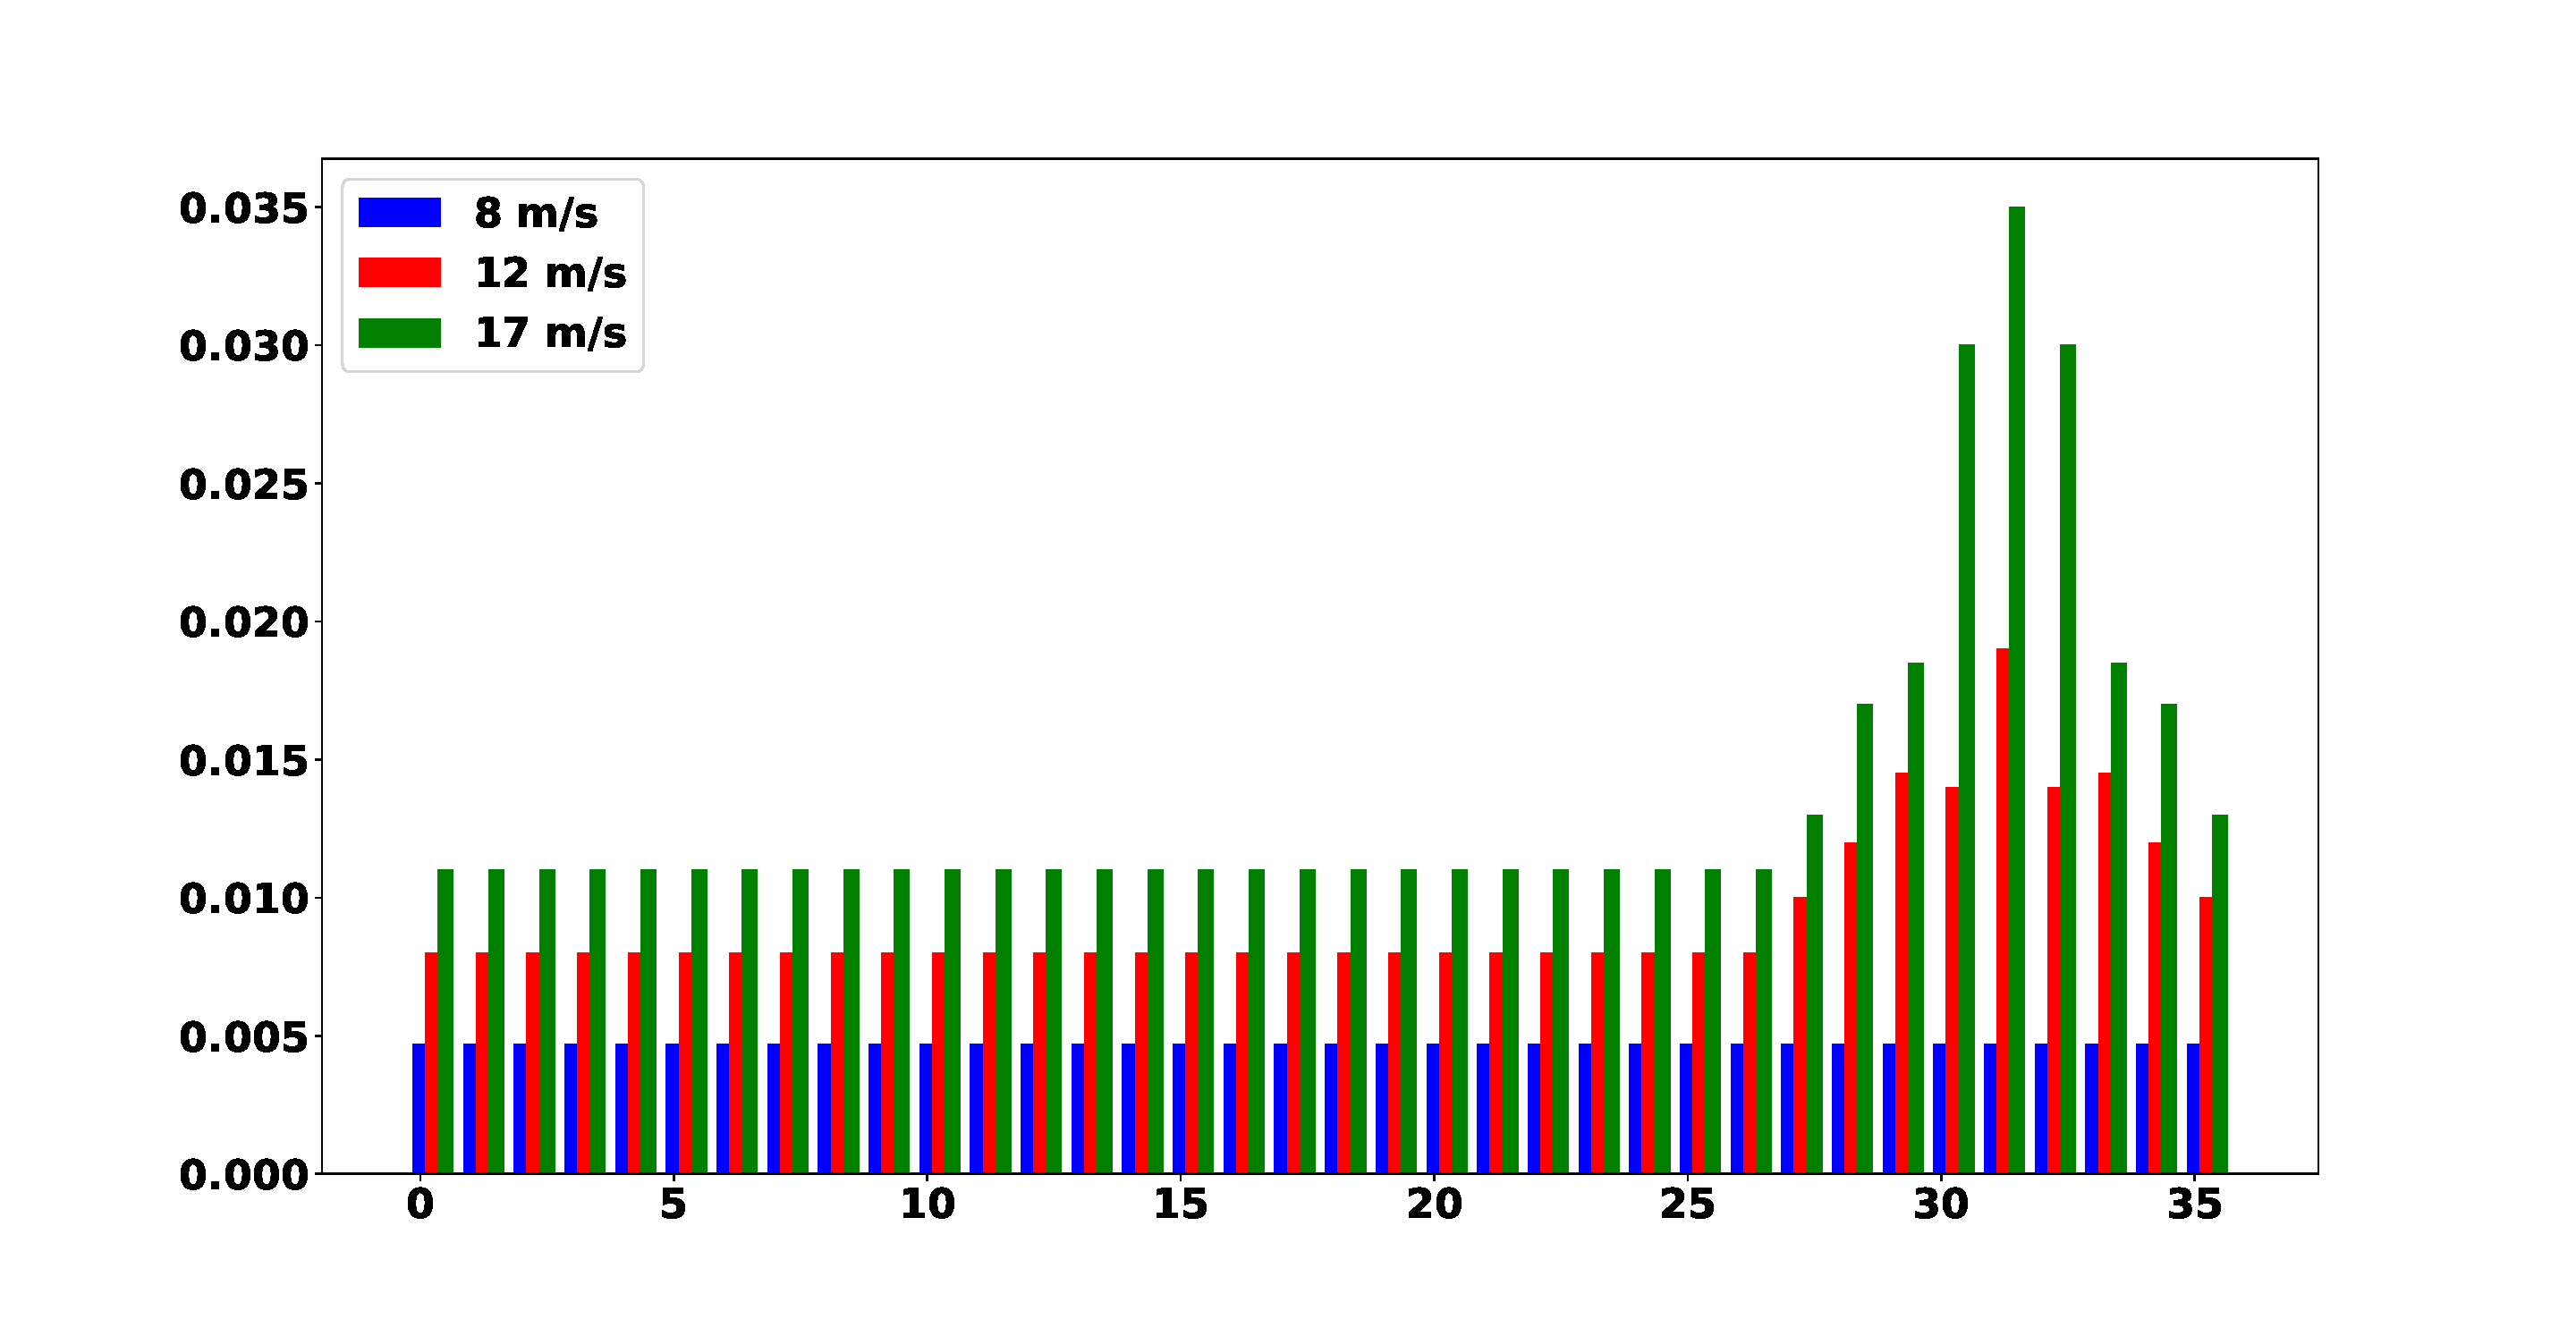
\includegraphics[scale = 0.3]{prob_wind_pdf.pdf}
	
	\caption{Wind regimes: x-axis is the angle (times 10 degrees), y-axis is the probability for wind regime, and color corresponds to free wind speed for the different wind directions.}\label{fig:prob_wind}
\end{figure}

\paragraph{Optimization Benchmarks}

We compared our two models, namely QCOP and QUBO, against two state of the art exact optimization methods:
the integer linear programming (ILP-LS) approach from~\cite{donovan2005wind}, and the 
model that uses a quadratic approximation (QP-SS)~\cite{turner2014new}. The CP approach presented in~\cite{Zhang2014} was
reported to perform worse than the rest and was left out of the experiments.
We used state of the art software, namely Gurobi~\cite{gurobi}, to solve QCOP, ILP-SS and QP-SS. 
We shall refer to the QCOP problem as QP-LS as it is a quadratic program that uses the LS objective.
In addition, we 
applied both Fujitsu's digital annealer and Gurobi to solve the QUBO variant of WFLO. We shall refer to the former as DA-LS, and to the latter
as QUBO-LS.


\paragraph{Experimental Procedure}

For exact methods (QP-SS, ILP-LS, QP-LS and QUBO-LS),
we ran Gurobi with a time limit of 3600 seconds. We collected all feasible solutions
until that point in time. The best solution in terms of energy is the solution that attained the highest objective
values (SS in QP-SS and LS in the rest of the methods).
For the digital annealer, we used a single configuration that was found to work best across the different instances \todo{Jason, please insert details about the DA config. here} The DA ran until convergence of the underlying simulated annealing algorithm and the runtime 
of the procedure was recorded. \todo{@Chris: do we want to share the code that ran the experiments in batches? perhaps it should be separated from the problem construction and the two need to be shared separately} 

The exact methods were all solved using Gurobi's quadratic programming solver on \todo{Jason, please add machine details here}. Furthermore, QUBO-LS was solved on DA version 1 \todo{Eldan: any additional info that we need to add here?}.

\paragraph{Performance Measurement} 

We have measured the total expected energy of a solution using the SS expression (see Eq.~(\ref{eq:ss}))\footnote{Note that the total mean energy is presented in kW.}.
The only method that optimizes on SS is QP-SS. Hence, for the other methods, we converted solutions
LS-based solution into the SS expression using Eq.~(\ref{eq:ss}) as proposed in~\cite{Zhang2014}. Specifically, let $x = (x_1, \ldots, x_k), k=n^2$ be a turbine placement solution obtained by an LS-based method.
Then, the SS based energy expression can be written as, 
$$\sum_{i\in \mathcal{N}}\sum_{d \in \mathcal{D}} \frac{1}{3} x_i \Bigg(u_{id,\infty} \Bigg[1-\sqrt{\sum_{j\in \mathcal{U}_{id}}x_j\bigg( 1-\frac{u_{ijd}}{u_{id,\infty}} \bigg) } \Bigg]    \Bigg)^3.$$ 

Next, we tested the performance of our approach as function of solution time. To this end, we 
compared the average performance of all WFLO methods on all 12 WFLO instances. Since energy levels are not directly comparable between the different instances (due to varying number of turbines and wind farm specs) we used the \emph{mean relative error} (MRE) measure. The MRE is defined with respect to the best solution obtained per instance and can be computed over time. Then, the
time-varying MRE can be averaged across the 12 scenarios and presented over time. In what follows, we demonstrate the construction of the MRE measure.

Recall that $\mathcal{W}$ is the set of our 12 standard WFLO instances. 
Moreover, we let $b_w$ be the best energy solution (in terms of SS) obtained for an instance $w \in \mathcal{W}$ 
across the different methods. For example, the best solution (within 3600 seconds) for the second instance $w_2$ that aims at placing $30$ turbines on a $10\times10$ grid with a single wind regime is attained by QUBO-LS and the SS energy expression is $15742$ (kW); thus, we set $b_w = 15742$. Then, for every point in time $t \in \{0,\ldots, 3600\}$ (measured in seconds), we can compute the relative error of a given approach per instance $w$. Let $\mathcal{A}$ be the set of solution approaches, $\mathcal{A}= \{QUBO-LS, QP-LS, DA-LS, ILP-LS, QP-SS\}$. Further, denote by $b_{w,t,a}$ denote the best solution attained before time $t$ of approach $a$ for instance $w$. Then, the mean relative error at time $t$ for approach $a$ on instance $w$ is given by \begin{equation}MRE(w,t,a) = \frac{b_{w,t,a}}{b_w}.\end{equation} We can now average over the different instances at time $t$. The average performance of approach $a$ at time $t$, $MRE(t,a)$ can be computed as, \begin{equation} MRE(t,a) = \frac{1}{|\mathcal{W}|}\sum_{ w\in\mathcal{W}} MRE(w,t,a).\end{equation}
We shall present $MRE(t,a)$ for each of the approaches to demonstrate the speed of convergence of the proposed LS-based methods. \todo{Jason: please check that this is consistent with how you calculated MRE in the experiment.} 


\subsection{Main Results}

In this part, we present the main findings of our empirical evaluation. 
We shall start by showing the best attained solutions by all methods.
Table~\ref{tab:results1} contains the best energy (in kW) attained by the methods
for the 12 WFLO instances after $100$ seconds of runtime for the exact methods. 
The runtime for DA-LS was always less than $10$ seconds.


\begin{table}[t!]
	
	\begin{tabular}{| c | c | c | c | c | c | c | c |}
		\toprule
		Wind Directions  & n  & m  & DA-LS  & QUBO-LS  & QP-LS  & QP-SS  & ILP-LS  \\
		\toprule
		\multirow{6}{*}{WR1}  & \multirow{3}{*}{10}       & 20       & \textbf{11185.41} & \textbf{11185.41}* & \textbf{11185.41}* & \textbf{11185.41}* & \textbf{11185.41}* \\
		& & 30   & 15740.69 & \textbf{15742.93}  & 15738.45  & 15735.1  & 15739.57     \\
		& & 40 & \textbf{19265.21} & 18952.97 & \textbf{19265.21}  & \textbf{19265.21} & \textbf{19265.21}                \\
		\cline{2-8}
		&\multirow{3}{*}{20}   & 20       & \textbf{11404.8}  & \textbf{11404.8}*  & \textbf{11404.8}*  & \textbf{11404.8}*  & \textbf{11404.8}*           \\
		&&30   & 16570.96 & 16715.19  & \textbf{16758.45}  & 16755.75 & 16695.05                  \\
		&&40   & 21874.04 & 21643.56  & 21905.5 & \textbf{21977.17} & \textbf{21977.17}        \\
		\hline
		\multirow{6}{*}{WR36} &  \multirow{3}{*}{10}    & 20       & \textbf{19221.44} & \textbf{19221.44} & \textbf{19221.44} & 19193.42 & 19022.77 \\
		&& 30  & \textbf{27450.99} & 27418.74 & 27442.9 & 27387.06 & 27247.5                     \\
		&&40   & 34888.81 & \textbf{34938.65} & \textbf{34938.65} & 34817.27  & 34671.62          \\
		\cline{2-8}
		&  \multirow{3}{*}{20}   & 20   & \textbf{19441.17}  & 19172.56 & 19336.33 & 19354.23  & 18448.64            \\
		&&30   & \textbf{27975.55} & 27443.8  & 27752 & 27492.11  & 26367.2                      \\
		&&40   & 35604.45 & 35127.32 & \textbf{35665.6}   & 35065.85 & 33451.94 \\
		\bottomrule                   
	\end{tabular}
	
	\vspace{0.5em}
	\caption{Total Expected Power (kW) after 100 seconds as function of benchmark and method. * denotes optimal solution. \todo{@Jason: could you please check if my marking of * for optimal solutions is correct? I think that optimality was proven only for $m=20$ and single wind direction, right?} }\label{tab:results1}
\end{table}


\begin{table}[t!]
	
	\begin{tabular}{| c | c | c | c | c | c | c | c |}
		\toprule
		Wind Directions  & n  & m  & DA-LS  & QUBO-LS  & QP-LS  & QP-SS  & ILP-LS  \\
		\toprule
		\multirow{6}{*}{WR1}  & \multirow{3}{*}{10}       & 20       & \textbf{11185.41} & \textbf{11185.41}* & \textbf{11185.41}* & \textbf{11185.41}* & \textbf{11185.41}* \\
		& & 30   & 15740.69 & \textbf{15742.93}  & 15738.45  & 15735.1  & 15739.57     \\
		& & 40 & \textbf{19265.21} & 18952.97 & \textbf{19265.21}  & \textbf{19265.21} & \textbf{19265.21}                \\
		\cline{2-8}
		&\multirow{3}{*}{20}   & 20       & \textbf{11404.8}  & \textbf{11404.8}*  & \textbf{11404.8}*  & \textbf{11404.8}*  & \textbf{11404.8} *          \\
		&&30   & 16570.96 & 16742.66  & 16758.45  & 16755.75 & \textbf{16770.2 }                 \\
		&&40   & 21874.04 & 21832.5  & 21963.81 & \textbf{21977.17} & \textbf{21977.17}        \\
		\hline
		\multirow{6}{*}{WR36} &  \multirow{3}{*}{10}    & 20       & \textbf{19221.44} & \textbf{19221.44} & \textbf{19221.44} & 19193.42 & 19213.96 \\
		&& 30  & \textbf{27450.99} & 27442.9 & 27442.9 & 27387.06 & 27389.21                     \\
		&&40   & 34888.81 & \textbf{34938.65} & \textbf{34938.65} & 34817.27  & 34856.45          \\
		\cline{2-8}
		&  \multirow{3}{*}{20}   & 20   & \textbf{19441.17}  & 19394.58 & 19336.33 & 19354.23  & 19368.86            \\
		&&30   & \textbf{27975.55} & 27785.74  & 27752 & 27492.11  & 27633.2                      \\
		&&40   & 35604.45 & 35480.9 & \textbf{35665.6}   & 35065.85 & 35210.78 \\
		\bottomrule                   
	\end{tabular}
	
	\vspace{0.5em}
	\caption{Total Expected Power (kW) after 3600 seconds as function of benchmark and method. * denotes optimal solution.}\label{tab:results2}
\end{table}


We observe that the DA-based solution provides
comparable results to state-of-the-art exact methods. For the harder instances (of $36$ wind directions),
the three quadratic LS-based approaches (DA-LS, QUBO-LS, and QP-LS) dominate the others by finding the best (or equal) solutions in 11 out of 12 instances. For easier instances, 
the linear approach (ILP-LS) finds better solutions \todo{@Chris, Jason: do we have a good explanation for this?}. Table~\ref{tab:results2} shows the same type of results as in Table~\ref{tab:results1}, but now after $3600$ seconds. We see that the DA is still competitive with the other approaches (recall, its solution was found after $10$ seconds),
while QP-LS finds the best solutions in 10 out of the 12 scenarios. For the 6 hard scenarios (12 wind directions), our quadratic solutions
dominate all 6. \todo{@Chris: I am not sure that the first table contributes anything beyond the second table}

We now turn to present the mean relative error over time per approach, i.e., we are presenting $MRE(a,t)$). Note that lower values indicate better performance.  Figure~\ref{fig:results1} 
presents the MRE after $50$ seconds of running the solutions focusing runtime performance, while Figure~\ref{fig:results2} corresponds
to the full run (after $3600$ seconds). The latter provides insights into best performance in terms of energy. The 5 different lines (and their colors) 
correspond to the 5 WFLO solutions. The horizontal axis represents time in seconds.


The results show that on average (across the 12 instances),
the ILP-LS method starts with poor solutions, yet ends up improving over QP-SS and QUBO-LS (after around 1250 seconds).

The two methods that are based on advanced software (QP-LS) and hardware (DA-LS) solutions
outperform the rest both in terms of runtime (best results in short time), and in terms of overall performance.
Specifically, for most instances, QP-LS gives the best solution at 3600 seconds, while the DA-based approach
yields competitive solutions after less than 10 seconds. Furthermore, QP-LS converges to the best solution faster than all other exact methods. In fact, it is inferior only to the approximate DA-LS method, which is geared mainly toward runtime. This is an encouraging result, especially due to the pessimistic computational complexity of WFLO.

\begin{figure}[t]%
	
	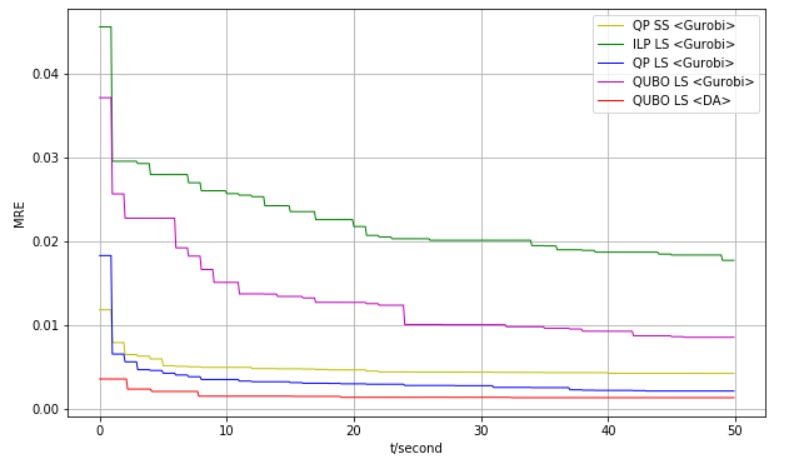
\includegraphics[width=\textwidth]{energy_50.png}  
	\caption{Mean Relative Energy (w.r.t. best feasible solution) vs. Runtime (after 50 seconds).}%
	
	\label{fig:results1}%
\end{figure}

uwo\begin{figure}[t]%
	
	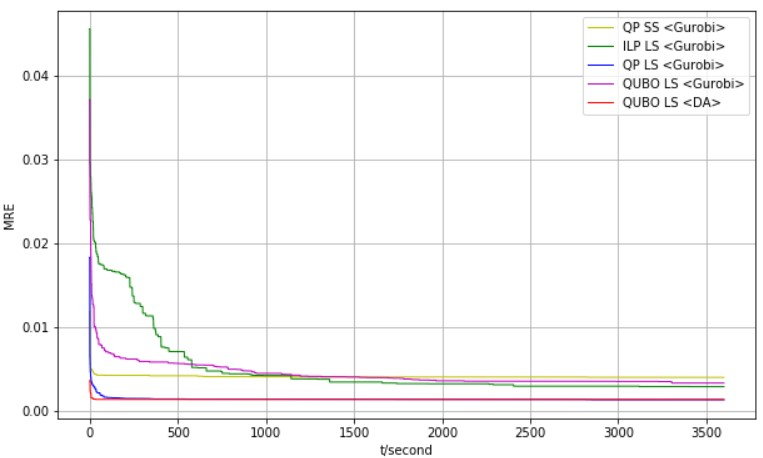
\includegraphics[width=\textwidth]{energy_3600.png}   \\%\\
	\caption{Mean Relative Energy (w.r.t. best feasible solution) vs. Runtime (after 3600 seconds).}%
	
	\label{fig:results2}%
\end{figure}



\subsection{Discussion}

Our result show empirically that the quadratic programming models that we
introduced in Section~\ref{sec:QUBO4WFLO} (QCOP and QUBO) are useful in two ways.
First, QCOP and QUBO are the basis for the QP-LS and QUBO-LS methods that couple
quadratic formulations of WFLO with Gurobi optimizer. This turns out
to be a powerful method as it gives the best performance after 3600 seconds for most instances (7 out of 12),
and especially,
for the hard instances with 36 wind directions. In addition, the runtime performance of QP-LS is second
only to the digital annealer.  
Second, the QUBO model can be mounted onto a quantum-inspired optimization hardware (e.g., Fujitsu's digital annealer) demonstrated by the DA-LS approach in our evaluation. DA-LS yields the best results in 7 out of 12 
instances, shows competitive performance on the other instances, and outperforms all methods in terms of runtime.

 
The ability of DA-LS to quickly obtain competitive solutions on large WFLO instances 
can be employed to solve
multiple wind farm design problems. This allows the flexibility to tune the various WFLO parameters (including turbine specs, number of turbines, and farm sizes) without incurring a steep computational cost that came
(so far) with re-solving the problem. In addition, the performance loss due to the use of an approximate method 
that uses advanced technology is negligible. This balance (instead of trade-off) between
runtime and total energy, points at the usefulness of the proposed quadratic formulations of WFLO.  \todo{maybe we should say some of these things in the intro and bring citations to the fact that demand for wind farms increases. I found some papers about surge in China and the UK.}
 


  
\section{Conclusion}
\label{sec:conclusion}

In this work, we presented a novel quadratic programming framework
for solving 
wind farm layout optimization. 
The framework is based on two models: a constrained model (QCOP) and an unconstrained binary
model (QUBO). The former can be used to solve WFLO with advanced optimization software,
while the latter can be mounted onto quantum-inspired dedicated hardware that can quickly (yet approximately) solve WFLO. We used the constrained quadratic formulation to prove 
that the computational complexity of WFLO is $\mathcal{NP}$-hard, a pessimistic result that 
was also noticed experimentally in~\cite{Zhang2014}. However,
our empirical evaluation shows that when advanced exact solvers like Gurobi~\cite{gurobi} are
coupled with our QCOP and QUBO models they can solve small WFLO instances to optimality in less than 3600 seconds.
We also show that when an advanced hardware is used with the QUBO representation of WFLO, even large instances can be solved quickly with no significant decrease in the total energy compared to state-of-the-art exact methods.
This runtime improvement and state-of-the-art performance in terms of the total energy of the resulting solutions makes our proposed quadratic framework useful for designing new wind farms, while multiple input parameters. 


In future work, we aim at extending our quadratic models to include additional 
WFLO aspects, such as noise, non-flat terrain and multiple objectives. 
Moreover, we wish to explore real-world wind farm design problems 
that may be larger and more complex than the 12 standard instances, and solve them 
using our quadratic programming approach. 

\bibliographystyle{elsarticle-num-names}
%\bibliographystyle{plainnat}
\bibliography{Biblio}

\end{document}



%
%\begin{table}[t]
%	
%
%	\label{tab:results1}
%	\vspace{-0.5em}
%	\scriptsize
%	\centering
%	\begin{tabular}{ c @{\hspace{1em}} c @{\hspace{1em}} c @{\hspace{1em}} c}
%		\toprule
%		Paper & Exact Optimization & Discrete Grid & Flat Terrain  \\
%		\midrule
%		\citet{Zhang2014,turner2014new} & + & + & +  \\
%		\citet{kuo2016wind} & + & + & -  \\
%		 \citet{} & + & - & + \\
%		
%		\bottomrule
%	\end{tabular}
%	\vspace{-1em}
%	\caption{Literature review of Wind Farm Optimization Layout solutions.}
%		
%\end{table}

